Las capturas y las salidas están en \cod{docs/evidencia/} y se pueden repetir con los mismos
comandos. Las de los roles se tomaron en el servidor local con la misma versión del código: en la
nube, iniciar sesión exige la contraseña y el código TOTP de cada personaje, que van en el anexo.

\subsection{El sistema por HTTPS}

\begin{salida}
\VerbatimInput{../evidencia/https.txt}
\end{salida}

\begin{figure}[H]
\centering
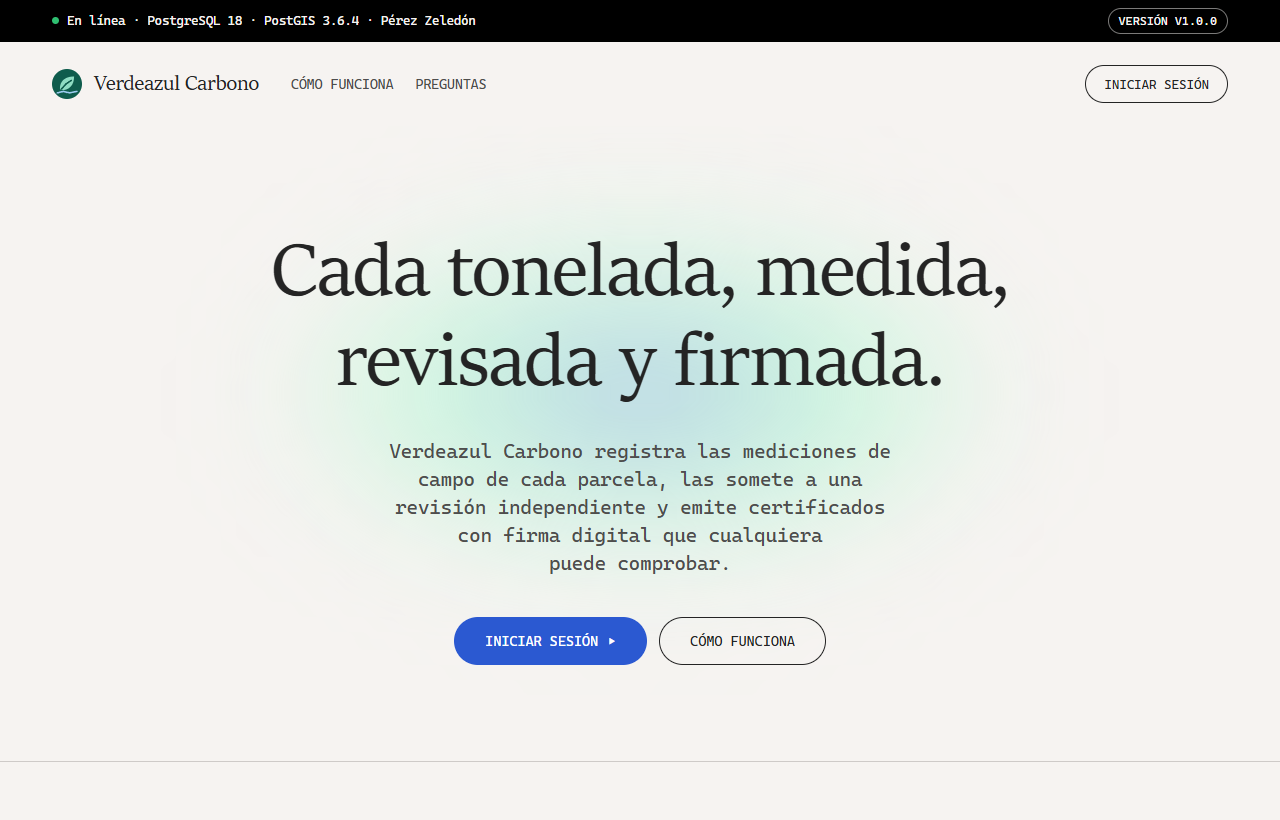
\includegraphics[width=0.42\textwidth]{../evidencia/01-app-https.png}
\caption{La portada de \cod{v1.0.0} en \url{https://verdeazul-app-708901712393.us-east1.run.app}. Las imágenes desplegadas y sus etiquetas, en el Anexo~B.}
\end{figure}

\subsection{Secret Manager}

\begin{salida}
\VerbatimInput{../evidencia/secret-manager.txt}
\end{salida}

\subsection{Dependabot activo}

\begin{figure}[H]
\centering
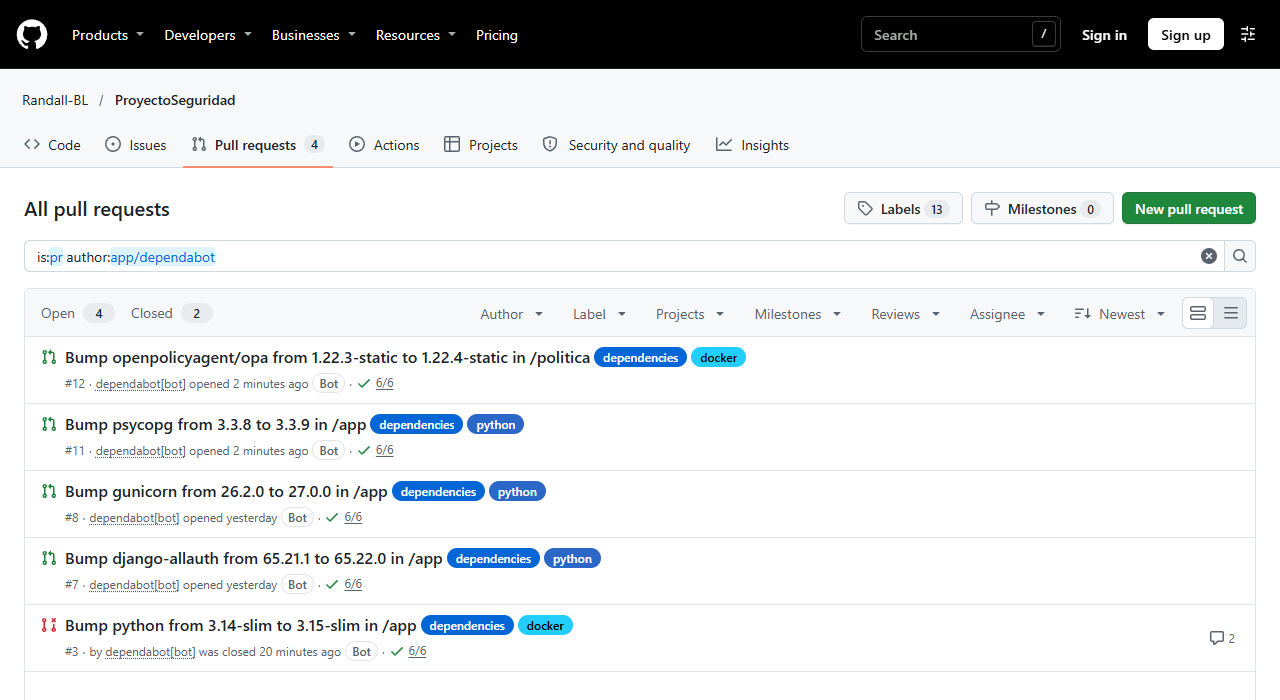
\includegraphics[width=0.55\textwidth]{../evidencia/05-dependabot-prs.png}
\caption{Las propuestas de Dependabot en el repositorio, el 15 de noviembre. El PR \#3 (Python 3.15)
se revisó y se cerró con la justificación escrita (tarea 9.2); las demás quedan para revisar con el
mismo procedimiento.}
\end{figure}

\subsection{Un certificado verificado y uno alterado}

\begin{figure}[H]
\centering
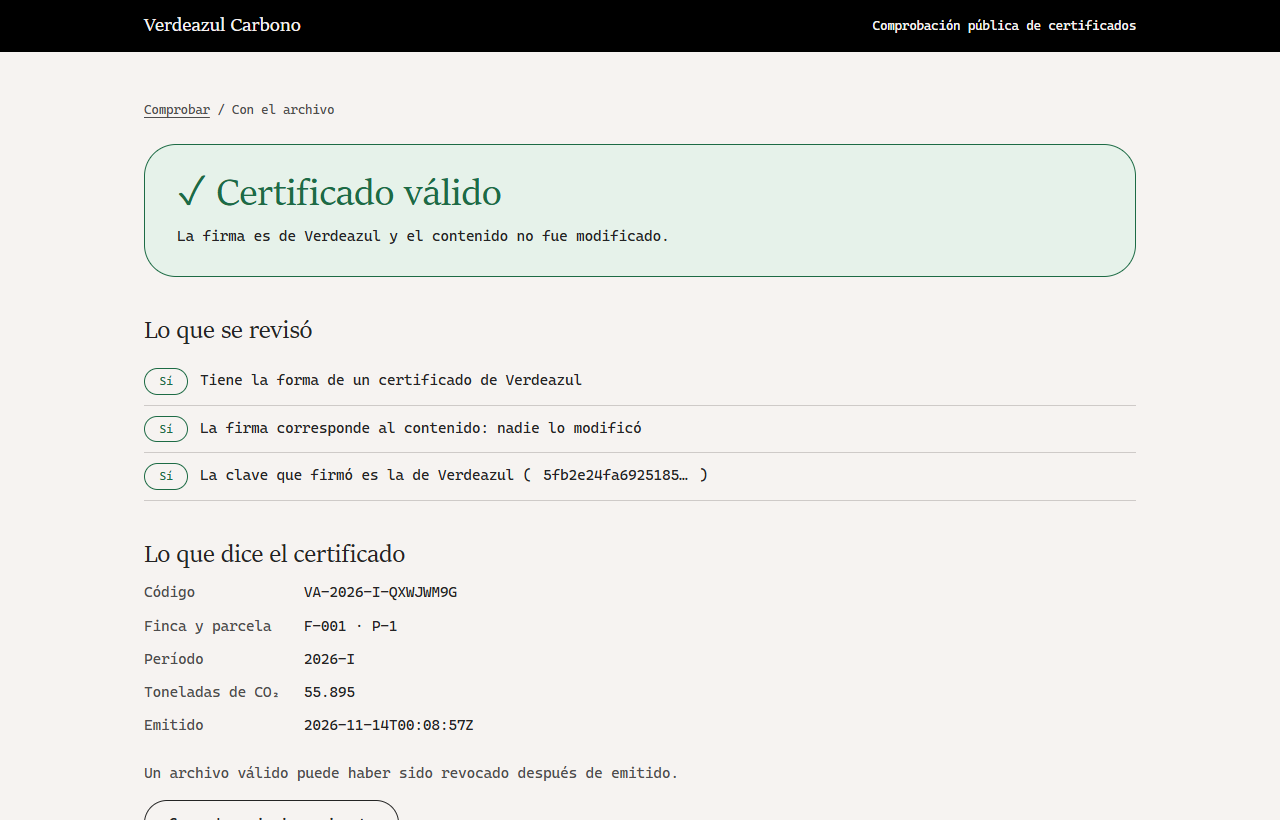
\includegraphics[width=0.49\textwidth]{../evidencia/02-certificado-valido.png}\hfill
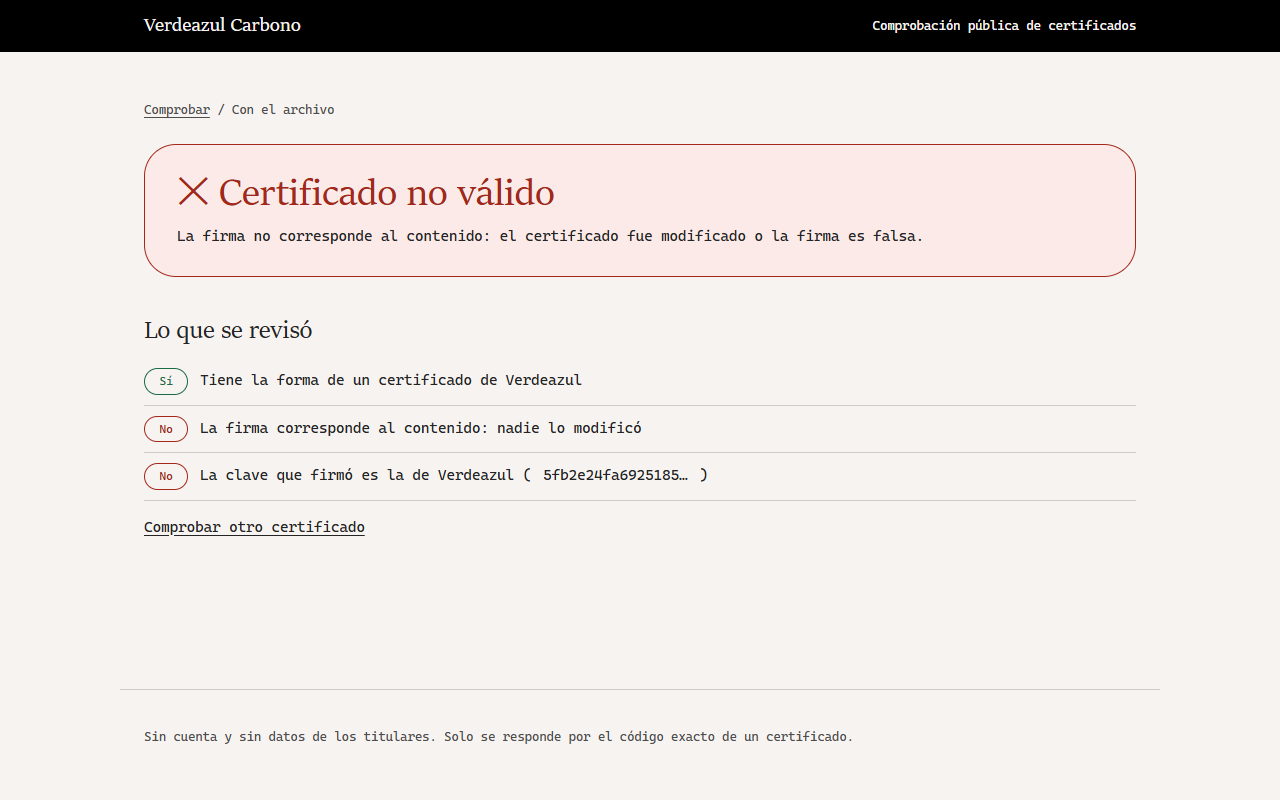
\includegraphics[width=0.49\textwidth]{../evidencia/03-certificado-alterado.png}
\caption{El servicio público con el certificado real \cod{VA-2026-I-QXWJWM9G} (izquierda) y con la
misma copia con una tonelada cambiada (derecha). Archivos en \cod{docs/demostracion/}; el verificador sin conexión da lo mismo (Anexo~B).}
\end{figure}

\subsection{El intento fallido de un rol}

\begin{figure}[H]
\centering
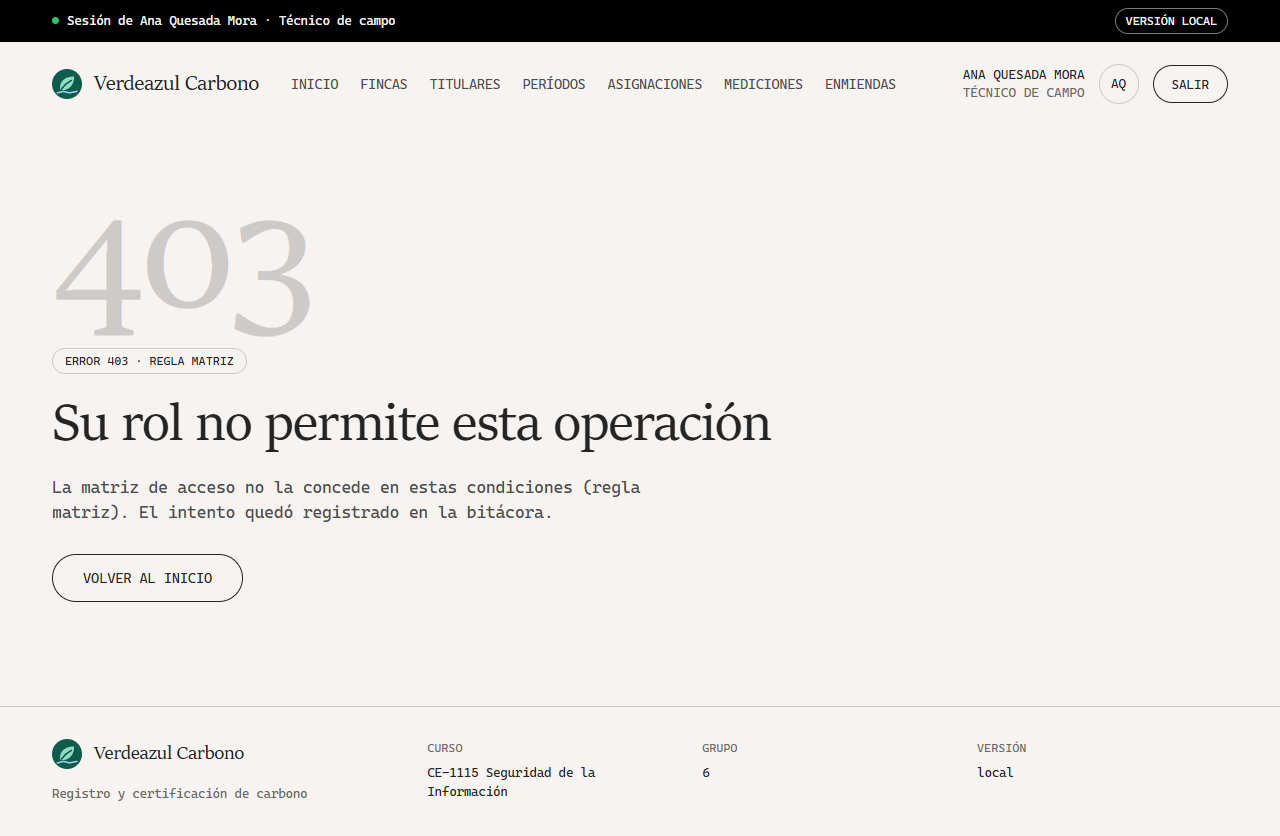
\includegraphics[width=0.49\textwidth]{../evidencia/06-tec-aprueba-sin-interfaz.png}\hfill
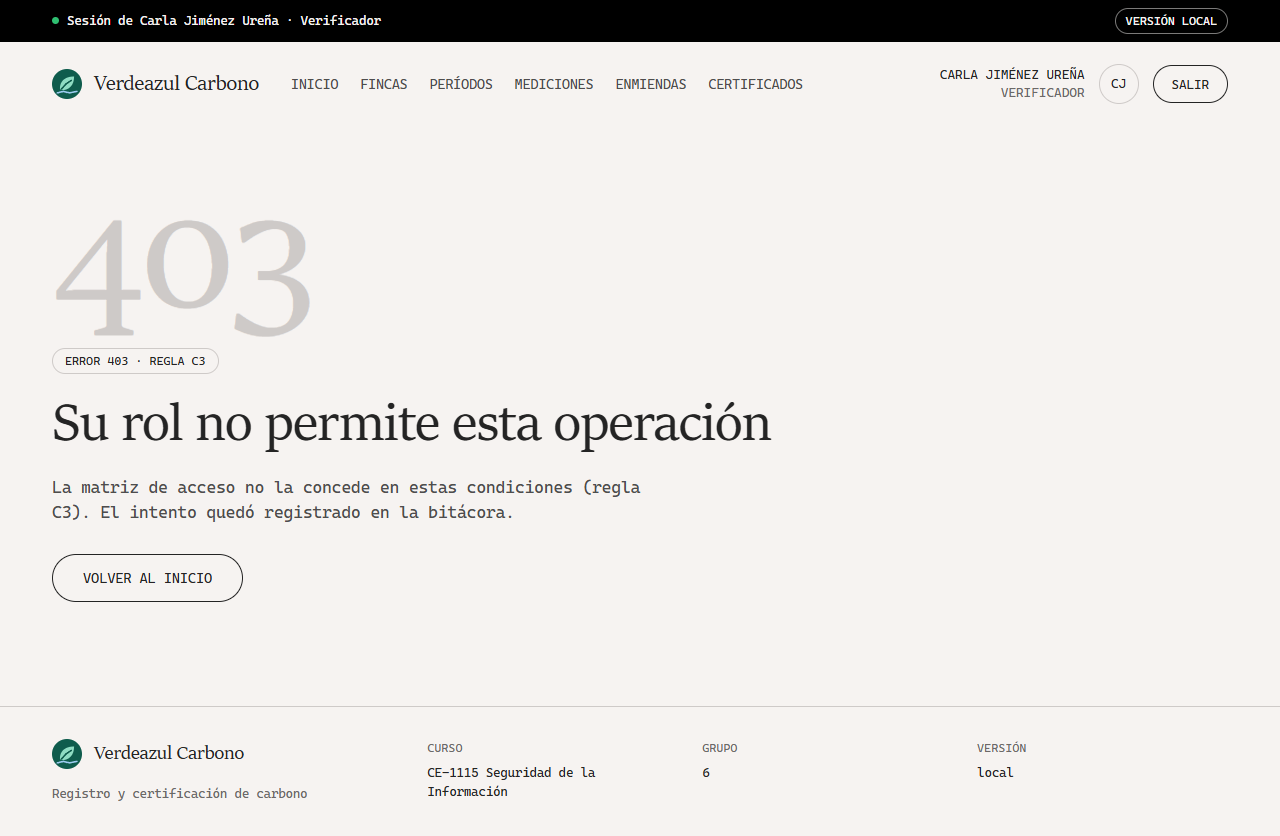
\includegraphics[width=0.49\textwidth]{../evidencia/07-ver-aprueba-lo-suyo-c3.png}
\caption{Izquierda: la técnica A envía a mano, con su sesión y su marca CSRF, la petición de aprobar
una medición; su rol no tiene ese verbo y el servidor la rechaza aunque la interfaz no muestre el
botón. Derecha: la verificadora C intenta aprobar una medición de la que escribió una versión: C3.}
\end{figure}

\begin{figure}[H]
\centering
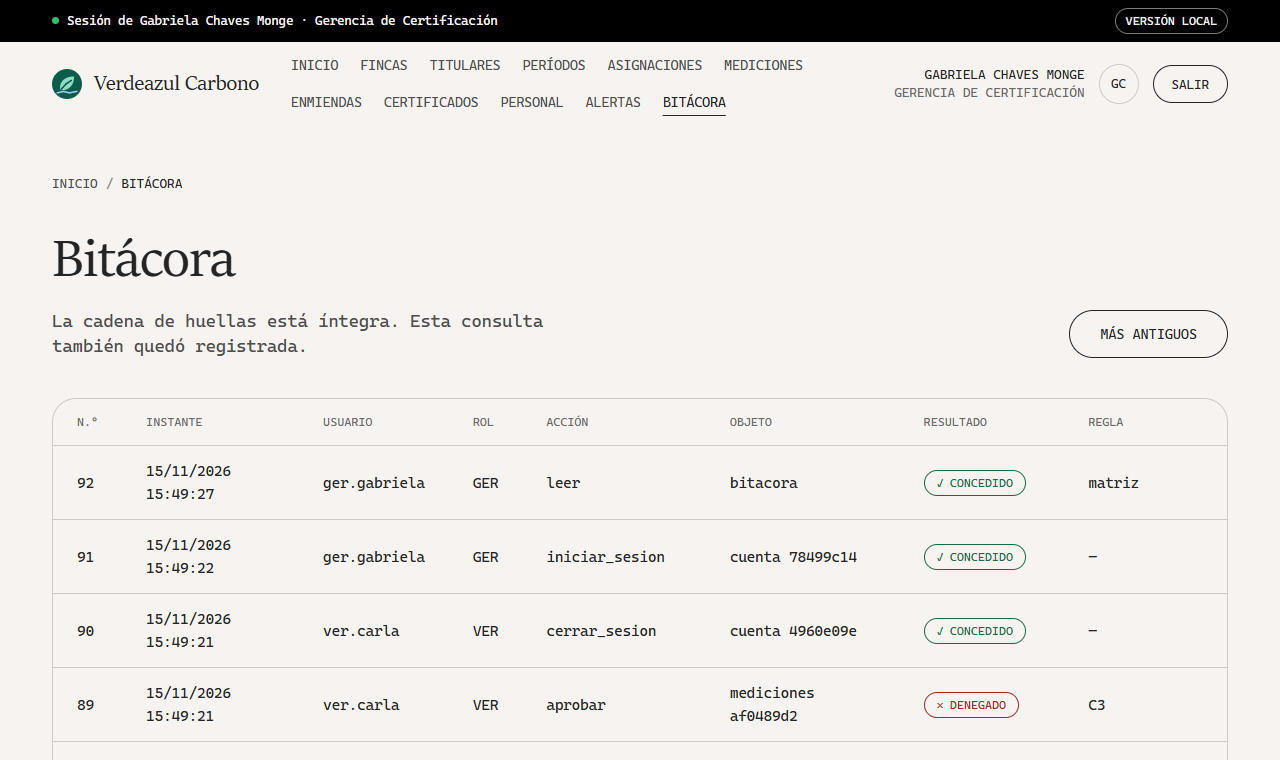
\includegraphics[width=0.5\textwidth]{../evidencia/08-bitacora-ger.png}
\caption{La bitácora vista por GER: los dos intentos quedaron como «denegado» con su regla (89: C3;
85: matriz), y la cadena de huellas está íntegra.}
\end{figure}
